\documentclass[../main/main.tex]{subfiles}

\begin{document}

\section{UML Class Diagrams}

The UML class diagram cheatsheet from \cite{oose:uml} is provided in the back.
A concise summary on the most important class notations, especially the
meanings of the different relationships and their use cases will be provided
below. 

\subsection{Relationships}

Instance level relationships comprise the association, aggregation and the
composition. 

Class level relationships are for instance, the generalization and the
realization. 

\subsubsection{Navigability}

Two quotes from \cite{umldiagrams:navigability} regarding the navigability. 

\begin{quote}
UML specification does not dictate how efficient this access should be or any
specific mechanism to achieve the efficiency. It is implementation specific.

When end property of association is marked as not navigable, in [UML 2.4] it
means that "access from the other ends may or may not be possible, and if it is,
it might not be efficient." The problem with this definition of not navigable is
that it actually means "whatever" or "who cares?" navigability.

\end{quote}

Their statement is also summarized in Figure \ref{fig:umlnav}.

\begin{figure}[h!]
  \centering
  \begin{subfigure}[b]{0.48\textwidth}
    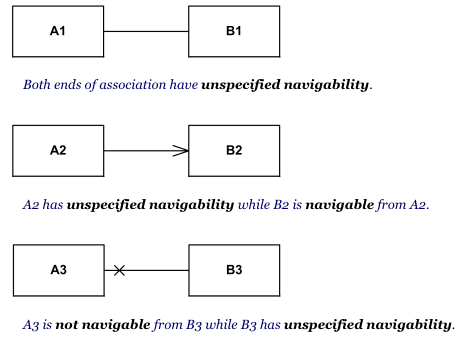
\includegraphics[width=\textwidth]{../figures/umlnav1.png}
  \end{subfigure}
  \begin{subfigure}[b]{0.48\textwidth}
    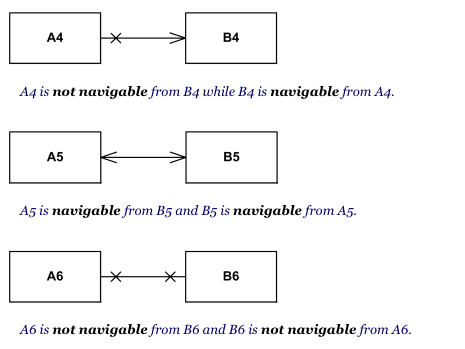
\includegraphics[width=\textwidth]{../figures/umlnav2.png}
  \end{subfigure}
  \caption{\cite{umldiagrams:navigability}}
  \label{fig:umlnav}
\end{figure}

\subsubsection{Association, Aggregation and Composition}

Association is the simplest in form as it merely represents a relationship
between two (or more) different classes. 

Aggregation is a binary relationship between two classes where the one contains
the other, however, if the container gets destroyed, the other class does not
necessairly have to be destroyed as well. 

Composition is, in contrast to aggregation, a lifecycle dependent relationship
between two different classes. 

Aggregation is more commonly used in software or database relationships, e.g.,
a class has a multitude of students. However, if the class gets destroyed, the
data of the students can still remain in the database. 

Composition is necessary if a real-world whole-part relationship should be
represented. The universe contains some stars, however, if it gets destroyed,
there will literally be a disaster (aster means star in Greek), as the stars
cannot exist without a universe. 

Scott W. Ambler says in \cite{ambler:composition}:

\begin{quote} 
  I'm a firm believer in the "part of" sentence rule -- if it makes
  sense to say that something is part of something else then there's a good
  chance that composition makes sense. For example it makes sense to say that a
  room is part of a building, it doesn't make sense to say that an address is
  part of a person. Another good indication that composition makes sense is when
  the lifecycle of the part is managed by the whole -- for example a plane
  manages the activities of an engine. When deciding whether to use composition
  over association, Craig Larman (2002) says it best: If in doubt, leave it out.
\end{quote}

\subsubsection{Generalization and Realization}

Generalization (dt. Vererbung) consists of the subtype and the superclass, where
each instance of the subtype is also an instace of the superclass. 

Realization happens if a class implements an interface class. 

\subsection{Association Class}

If we are dealing with a scenario where a participant takes part in a
competition. Then we could have an association class between them, e.g. a
class that stores the result of the participation. 


\subsection{Template Classes}

Templated classes, as we know from C++ (\lstinline|template<T>|) or Java
(Generics),can be represented by having a small box as show in the following
figure. 

The classes that implement this with a special template type, must also indicate
the type with a \lstinline|bind (i -> type)|.

\begin{figure}[h!]
  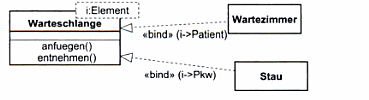
\includegraphics[width=0.5\textwidth]{../figures/umltemplate.png}
  \caption{Template from \cite{oestereich:kurzreferenz}}
\end{figure}

% from this beast source https://books.google.at/books?id=wS2PwGG6GNUC&pg=PA53&lpg=PA53&dq=parametrisierbare+klasse&source=bl&ots=B6dpTCtuYu&sig=1NiL0SUDN84LVh5biCeKg9MTCl0&hl=de&sa=X&ei=qaQuVa71Acm4acv8gZAD&ved=0CB8Q6AEwAA#v=onepage&q=parametrisierbare%20klasse&f=false

\subsection{Members and Scopes}

For the sake of completeness, the visibility can be represented with the
following characters: 

\begin{itemize}
  \item[] \lstinline|+| Public
  \item[] \lstinline|-| Private
  \item[] \lstinline|#| Protected
  \item[] \lstinline|~| Package
  \item[] \lstinline|/| Derived (e.g.\lstinline|/age : int {age = today - birthdate}|)
\end{itemize}

Static variables, or classified members, must be \underline{underlined}, while instance
members are assumed per default.

\subsection{Class Structure}

As depicted in the following figure:

\begin{figure}[h!]
  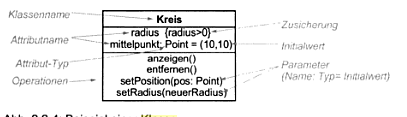
\includegraphics[width=0.5\textwidth]{../figures/class.png}
  \caption{Template from \cite{oestereich:kurzreferenz}}
\end{figure}

\subsection{Abstract vs Interfaces}

General thumb rule: If the class we are talking about should \textbf{be capable
of} doing something that a class requires, then we use realization (interfaces).
If the class \textbf{is a} something, then prefer abstract classes. 

% todo: when to use abstract vs interfaces

\subsection{Abstract Classes}

If the UML class diagram is drawn on paper, cursive text is hard to represent,
however, we can use the short notation \lstinline|{A}| to represent it.  

\subsection{Cheat Sheet}

\begin{figure}
  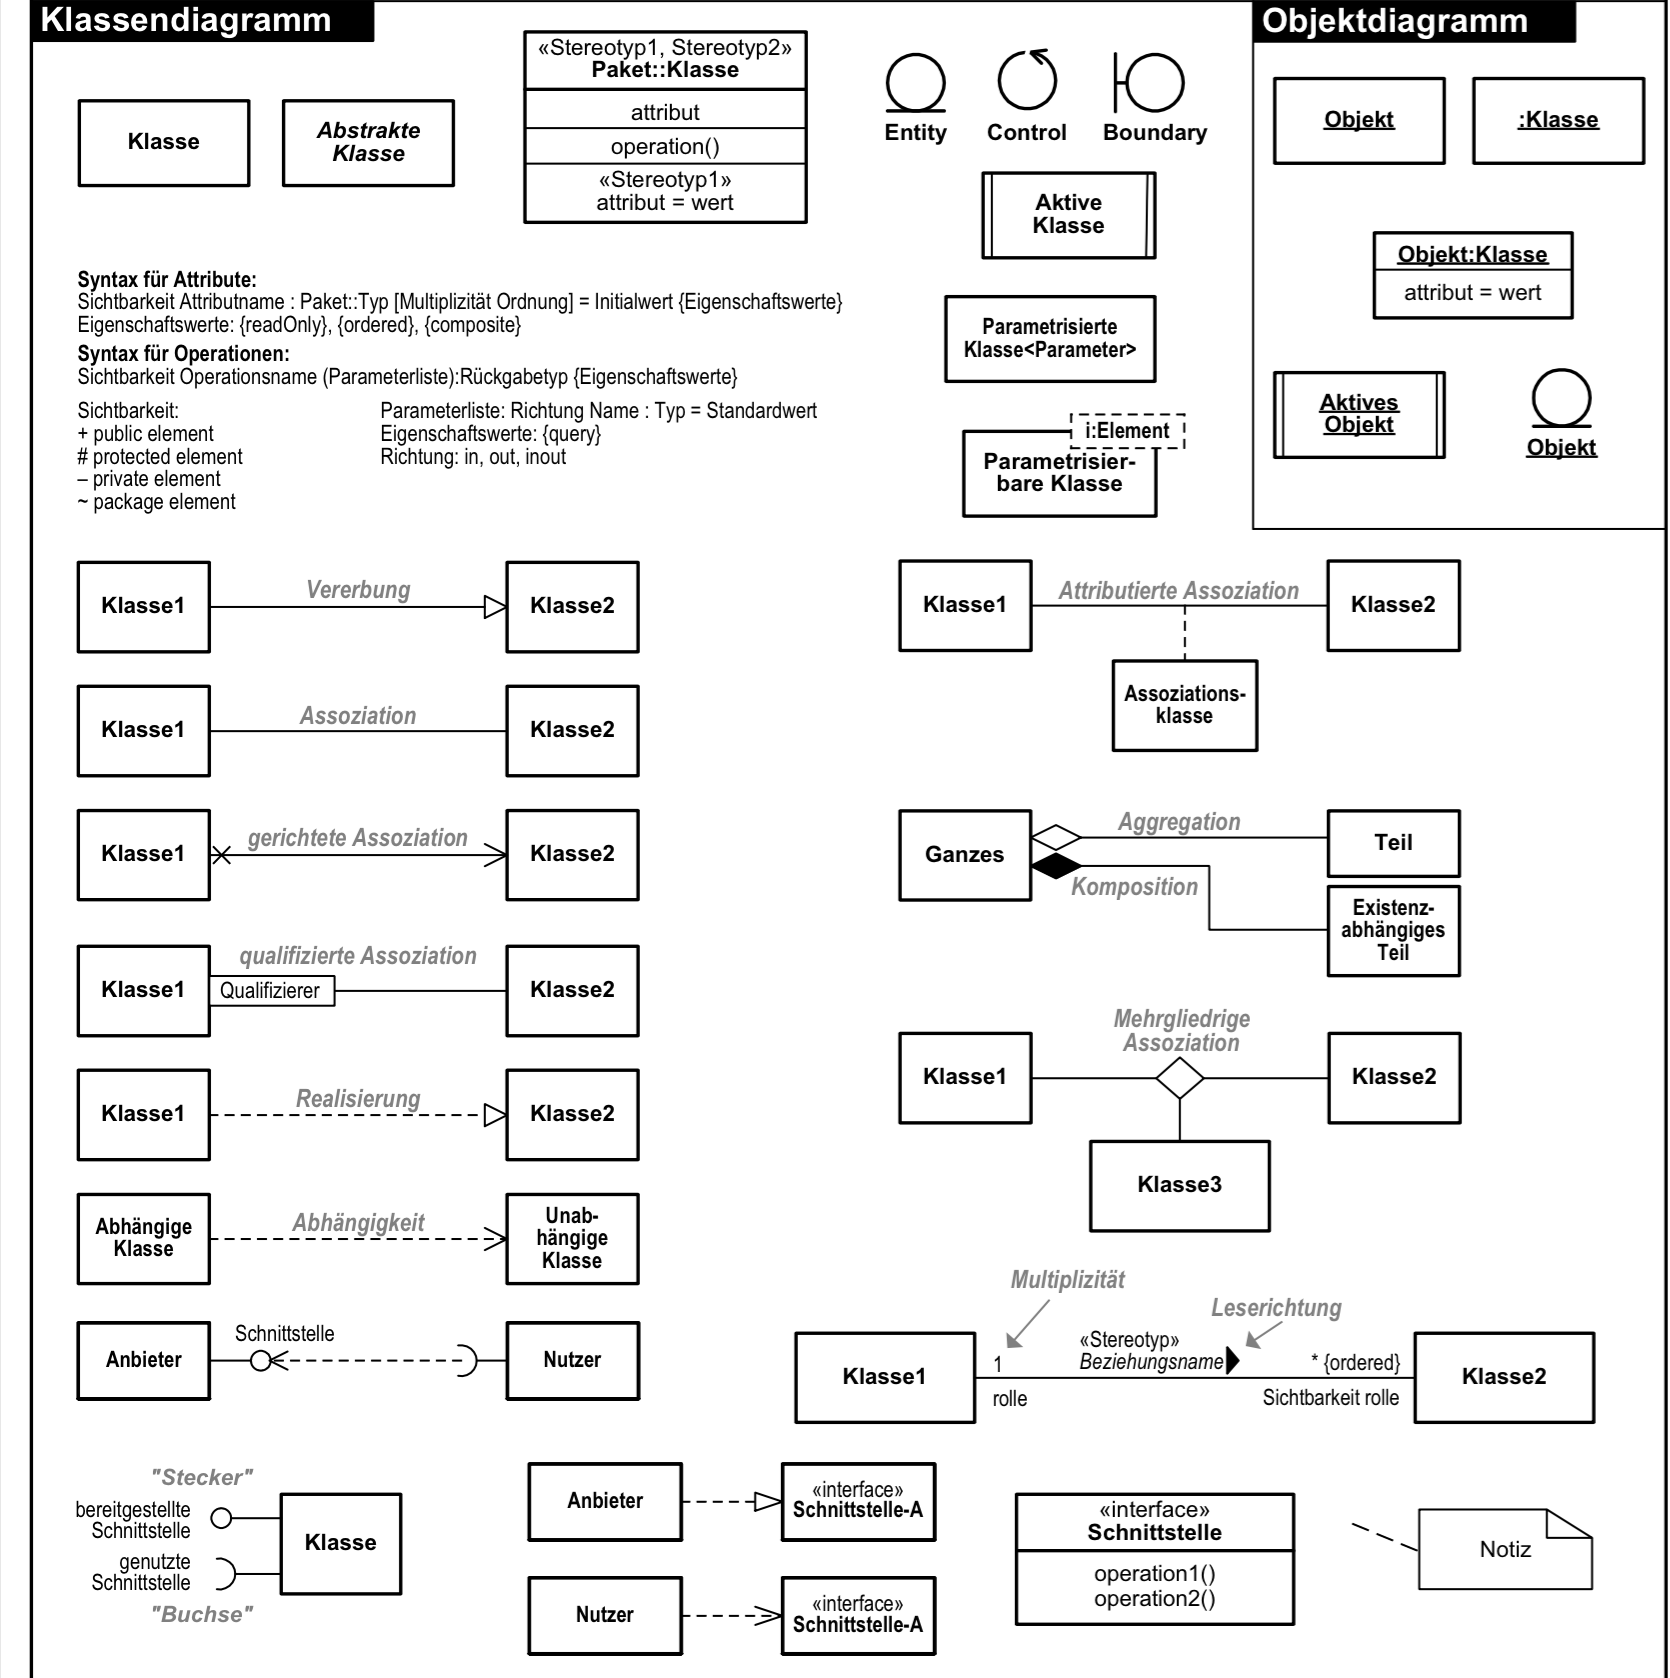
\includegraphics{../figures/uml_oose.png}  
  \caption{UML Oose \cite{oose:uml} }
  \label{fig:uml_oose}
\end{figure}

\end{document}
